\section{Empirical Results: Fixed Effects Regressions}
\label{app:FE_CRVE}


Our dataset includes a small set of explanatory variables, all of which are categorical. 
Also, the dataset is very large: it comprises several billion driver days. 
On the other hand, the dataset is very sparse, 
which lends itself to methods of aggregation and
econometric models that can be computed with frequency-weighted observations.
Drivers rarely get tickets, so that most observations represent zero tickets, 
resulting in many thousands of equivalent observations with many similar drivers 
receiving no ticket on a given day. 
Furthermore, we observe many instances in which several drivers 
get tickets with the same point value on a particular day, 
all of whom are in a single category, 
e.g. all males, aged 20-24, with two demerit points on their driving record. 
This drives the aggregation method that we followed in the main text, 
retaining the weekday and month categories and aggregating over the number of drivers. 
In this appendix, we investigate a model with fixed effects and cluster-robust standard errors, 
both calculated over the individual drivers. 

Estimating fixed effects for the individual drivers accounts for all the variation explained by age, sex and other unobserved heterogeneity between the drivers.
The demerit point balance is the only remaining variable that changes over time for a particular driver. 
% 
This categorical variable is defined as the sum of all points on tickets that a driver has received within the last two years. 
It is designed to reflect the demerit points that remain on a particular driver's record, 
which is taken into account when this balance reaches thresholds to warrant suspension or revocation of the driver's license. 
We calculate this balance including the two-year period before the sample start date of 01 April 2006, to ensure that the measurement is consistent across drivers and throughout the sample. 
Note, however, that this variable is closely related to lagged values of the dependent variable, 
whether a ticket occurred, so there is no reason to expect that the estimates are unbiased. 
The main reason to conduct this sensitivity analysis is to gauge the effect of
calculating standard errors clustered on individual drivers
with driver-specific fixed effects. 


\subsection*{All Drivers (with both high and low past demerit points)}


We estimated the fixed effects model with indicators for each demerit point category
and the interactions of these demerit point indicators with the period after the policy change. 
% 
The coefficients on the indicators for demerit point categories were largely insignificant for 
all samples considered in Table \ref{tab:FE_regs_CRVE_all_pts}, 
along with the coefficients for the interaction terms. 
% 
The point estimates of these effects, however, are similar for male and female drivers, 
and the coefficients are largely increasing in the number of demerit points. 
% 
% Note that the indicator is missing for the category of drivers with zero demerit points, 
% which is the benchmark group.
% 
We show only the interaction between the policy effect and demerit points
in Figure \ref{fig:FE_regs_all_pts}. 
% 
% 
We plotted the sum of the coefficients for these interactions and the policy indicator
to capture the net effect of the policy for each group of drivers.
% 
We also plotted 95\% confidence intervals for each sum of coefficients, 
for which the standard errors are calculated using the standard formula to take into account the variance of both policy coefficients and the covariance of the two.  
The standard errors of the individual coefficients were calculated with the cluster-robust variance estimator, 
in which the clusters were taken to be the individual drivers. 

Not much of an effect is apparent, whether for male or female drivers, with six or fewer demerit points, 
and the effect is only slightly stronger for drivers with between seven and ten demerit points. 
For drivers with more than ten demerit points, however, the relationship is much more pronounced. 
Drivers with ten to twenty demerit points are expected to get two fewer tickets per thousand driver days
under the excessive speeding legislation. 
For drivers with more than thirty demerit points, 
this number is as high as four tickets per thousand days---slightly more than one ticket per year---%
after the policy change. 
% 
Note that these values are much larger in magnitude than those in the text%
---we multiplied the coefficients by 100,000 driver days---%
compared to this analysis, the coefficients are on the order of ten or one hundred times as large. 
Although the results support the notion that drivers with high point balances were more strongly influenced by the policy, 
one must be cautions in interpreting these values in light of the bias induced
by the fact that the demerit points are essentially a moving average of a 
variable closely related to the dependent variable. 


\begin{figure}
\centering
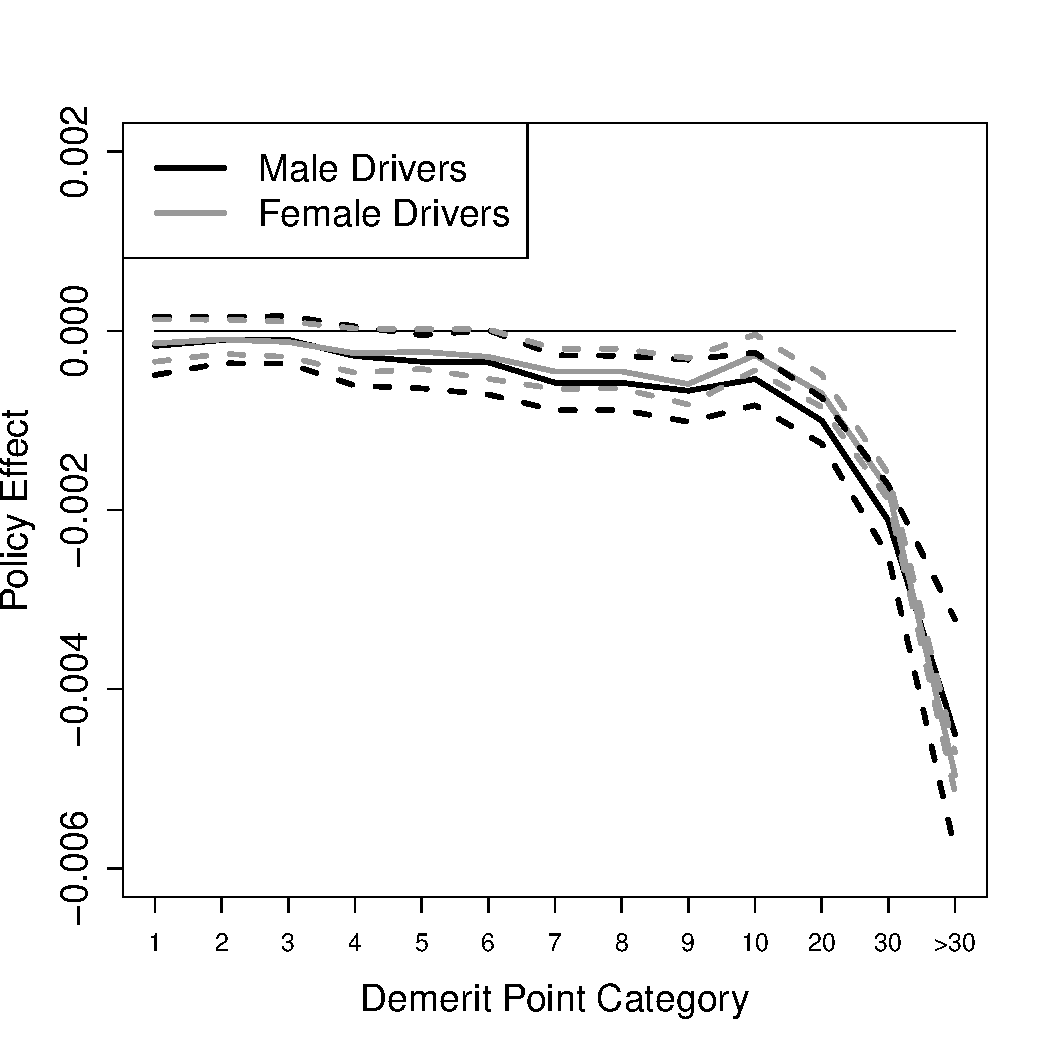
\includegraphics[width=0.8\textwidth]{Figures/FFX_reg_policy_points_grp_all_pts.pdf}
\caption{Policy change and demerit points group interactions (all drivers).
Solid lines represent the policy effect for drivers for each demerit-point category, 
calculated as the sum of the policy indicator and the interaction of the  indicators for the policy change 
and the demerit point category.  
Male drivers are represented by black lines and female drivers with grey. 
Dashed lines represent 95\% confidence intervals, 
calculated using cluster-robust standard errors, clustered on individual drivers. 
All estimates were calculated by fitting a fixed effects regression model, 
with intercept coefficients for each driver. 
}\label{fig:FE_regs_all_pts}
\end{figure}






\subsection*{High-Point Drivers}


We then studied the sample that is restricted to drivers with a history of getting tickets. 
We calculated balances of demerit points over rolling windows of two-year periods 
in the sample before the four-year window around the policy change. 
This way, we calculated 
the number of demerit points on each driver's record over the past two years, 
for all days from 01 April 2002 to 31 March 2006, which is the four-year period before the sample. 
Using this approach, we ensured that none of the tickets that were counted in those balances were included in the dataset for the regression model. 
We defined the sample of high-point drivers to include all drivers with six or more points during this pre-sample period. 


Figure \ref{fig:FE_regs_high_pts} depicts
the net effect of the policy indicator and the interaction of the policy 
indicator with the points group indicator for drivers with high point balances. 
First of all, the effects are very similar for males and females, aside from a slight difference among 
drivers with nine demerit points. 
Perhaps more striking is how narrow the confidence intervals are for drivers with a past record of demerit points. 
The policy effect is not very strong for drivers with three points or less but this 
relationship declines steadily for drivers with more demerit points. 
As with the full sample of drivers, the relationship takes a sharp downturn for drivers
with more than ten points. 
The level of the effect is similar to that measure on the sample of drivers with all point levels:
from a decrease of one ticket every three years to one ticket per year. 
Again, these numbers are much larger in magnitude than those we measured in 
the models without fixed effects
and should be interpreted with caution. 

\begin{figure}
\centering
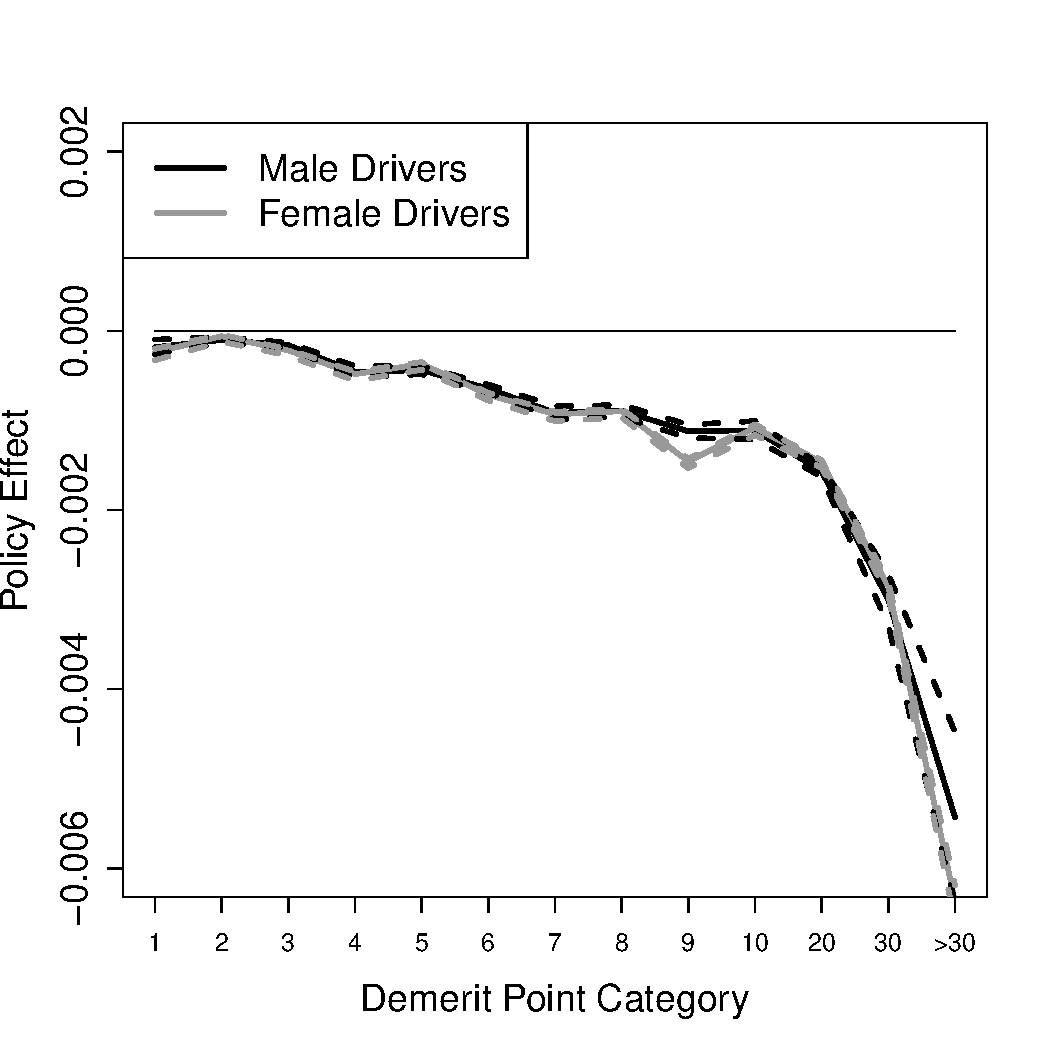
\includegraphics[width=0.8\textwidth]{Figures/FFX_reg_policy_points_grp_high_pts.pdf}
\caption{
Policy change and demerit points group interactions (drivers with high demerit points).
Solid lines represent the policy effect for drivers for each demerit-point category, 
calculated as the sum of the policy indicator and the interaction of the  indicators for the policy change 
and the demerit point category.  
Male drivers are represented by black lines and female drivers with grey. 
Dashed lines represent 95\% confidence intervals, 
calculated using cluster-robust standard errors, clustered on individual drivers. 
All estimates were calculated by fitting a fixed effects regression model, 
with intercept coefficients for each driver. 
}\label{fig:FE_regs_high_pts}
\end{figure}

